\documentclass[compress,11pt]{beamer}
%\includeonly{pendel}
\usetheme{Ilmenau}
%\usetheme{fau-4-3}
%\usecolortheme{beaver}
\beamertemplatenavigationsymbolsempty
\usepackage[ngerman]{babel}
\usepackage{marvosym}
\usepackage{multimedia}
\usepackage[utf8]{inputenc}
\usepackage{amsmath}
\usepackage{amsfonts}
\usepackage{amssymb}
\usepackage{graphicx}
\usepackage{esvect}
%\author{}
\title{EP Gruppe 8}
%\setbeamercovered{transparent}
%\setbeamertemplate{navigation symbols}{}
%\logo{}
%\institute{}
%\date{}
%\subject{}
\usepackage{verbatim}
\begin{document}

\begin{frame}

Schaltbild Filter 2. Ordnung, Erste Stufe:\\
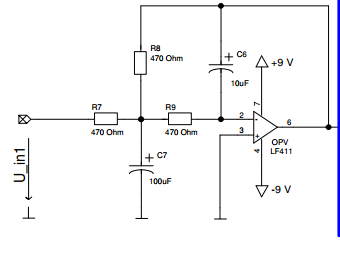
\includegraphics[width=.7\textwidth]{schalt/schalt_41}

\end{frame}

\begin{frame}
\begin{block}{Eigenschaften des Tschebyscheff-Filters}
\begin{itemize}
\item Im Vergleich zum passiven Filter 2. Ordnung: Einsatz vim Operationsverstärkern(Filter daher auch aktiv genannt)
\item Verlauf des Bode-Diagramms entspricht Tschebyscheff-Polynomen
\item daher im Bereich der Grenzfrequenz auch kein Monotoner Verlauf, sondern Welligkeit
\end{itemize}

\end{block}
\end{frame}

\begin{frame}
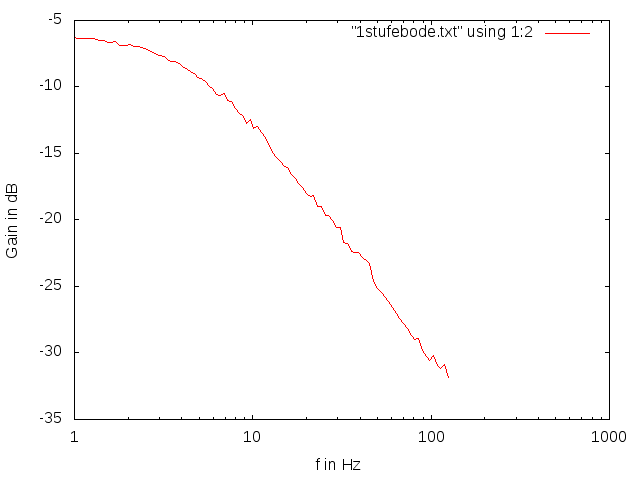
\includegraphics[width=.7\textwidth]{4aufgabe/1stufegain}\\
Gain-Bodediagramm der ersten Stufe
\end{frame}
\begin{frame}
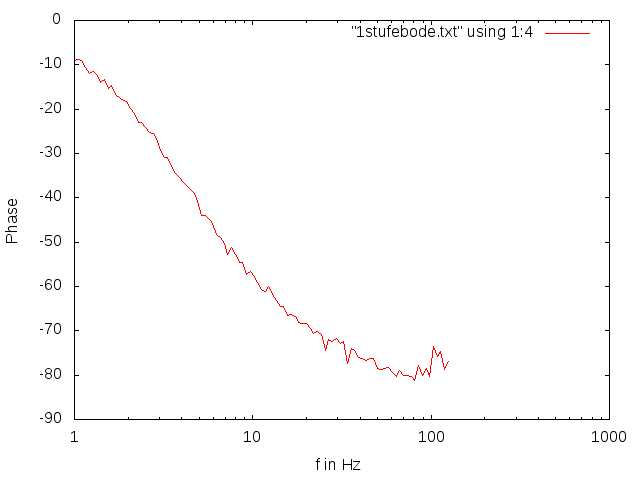
\includegraphics[width=.7\textwidth]{4aufgabe/1stufephase}\\
Phase-Bodediagramm der ersten Stufe
\end{frame}



\begin{frame}
Schaltbild Filter 2. Ordnung, Zweite Stufe:\\
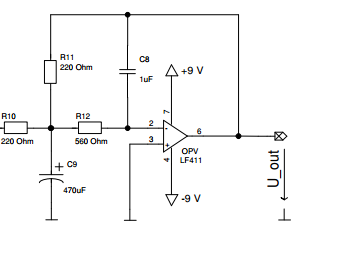
\includegraphics[width=.7\textwidth]{schalt/schalt_42}
\end{frame}




\begin{frame}
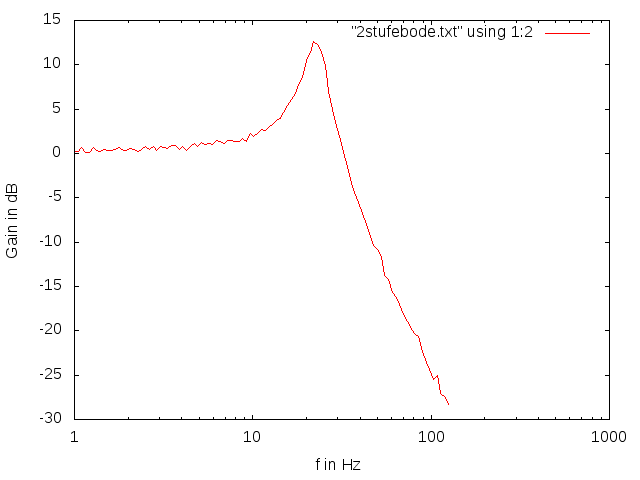
\includegraphics[width=.7\textwidth]{4aufgabe/2stufegain}\\
Gain-Bodediagramm der zweiten Stufe
\end{frame}
\begin{frame}
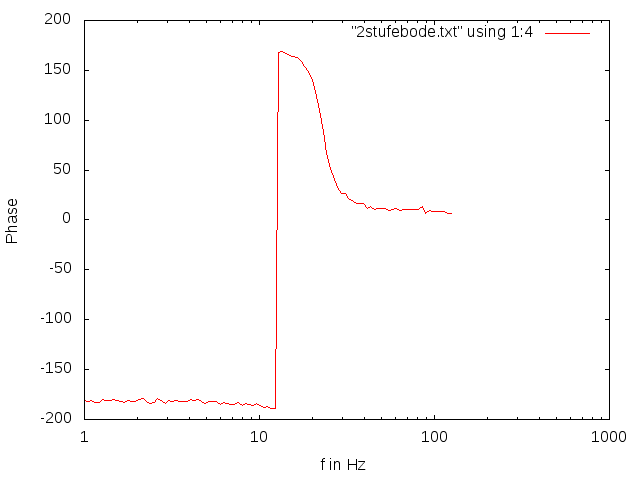
\includegraphics[width=.7\textwidth]{4aufgabe/2stufephase}\\
Phase-Bodediagramm der zweiten Stufe
\end{frame}

\end{document}